%%%%%%%%%%%%%%%%%%%%%%%%%%%%%%%%%%%%%%%%%%%%%%%%%%%%%%%%%%%%%%%%%%%%%%%%%%%
%                                                                         %
%			TEMPLATE LATEX PER TESI                                       %
%			______________                                                %
%                                                                         %
%           Ultima revisione: 24 giugno 2019                              %
%           Revisori: G.Presti; L.A.Ludovico; F. Avanzini                 %
%                                                                         %
%%%%%%%%%%%%%%%%%%%%%%%%%%%%%%%%%%%%%%%%%%%%%%%%%%%%%%%%%%%%%%%%%%%%%%%%%%%

\documentclass[12pt,italian]{report}
\usepackage{tesi}

%
%			INFORMAZIONI SULLA TESI
%			DA COMPILARE!
%

% CORSO DI LAUREA:
\def\myCDL{Corso di Laurea triennale in\\Informatica}

% TITOLO TESI:
\def\myTitle{Un Template \LaTeX\ per Elaborati\\Triennali o Tesi Magistrali}

% AUTORE:
\def\myName{Giorgio Presti}
\def\myMat{Matr. Nr. 662605}

% RELATORE E CORRELATORE:
\def\myRefereeA{Prof. Luca Andrea Ludovico}
\def\myRefereeB{Prof. Federico Avanzini}

% ANNO ACCADEMICO
\def\myYY{2018-2019}

% Il seguente comando introduce un elenco delle figure dopo l'indice (facoltativo)
%\figurespagetrue

% Il seguente comando introduce un elenco delle tabelle dopo l'indice (facoltativo)
%\tablespagetrue

%
%			PREAMBOLO
%			Inserire qui eventuali package da includere o definizioni di comandi personalizzati
%

% Package di formato
\usepackage[a4paper]{geometry}		% Formato del foglio
\usepackage[italian]{babel}			% Supporto per l'italiano
\usepackage[utf8]{inputenc}			% Supporto per UTF-8
%\usepackage[a-1b]{pdfx}			% File conforme allo standard PDF-A (obbligatorio per la consegna)

% Package per la grafica
\usepackage{graphicx}				% Funzioni avanzate per le immagini
\usepackage{hologo}					% Bibtex logo with \hologo{BibTeX}
%\usepackage{epsfig}				% Permette immagini in EPS
%\usepackage{xcolor}				% Gestione avanzata dei colori

% Package tipografici
\usepackage{amssymb,amsmath,amsthm} % Simboli matematici
\usepackage{listings}				% Scrittura di codice

% Package ipertesto
\usepackage{url}					% Visualizza e rendere interattii gli URL
\usepackage{hyperref}				% Rende interattivi i collegamenti interni
\usepackage{algorithm}
\usepackage[noend]{algpseudocode}
\usepackage{amsmath}
\usepackage{amsfonts}
\usepackage{verbatimbox}

\setcounter{secnumdepth}{3}
\setcounter{tocdepth}{3}
\begin{document}

% Creazione automatica del frontespizio
\frontespizio
\beforepreface

% 
%			PAGINA DI DEDICA E/O CITAZIONE
%			facoltativa, questa è l'unica cosa che dovete formattare a mano, un po' come vi pare
%

{\raggedleft \large \sl Questo lavoro \`{e} dedicato a tutti gli studenti\\
	
	\vspace{2cm}
	
	``Io studio,\\ma studiate pure voi,\\che se studio solo io non serve a un c\dots o''
	
	\bigskip
	
	\--- Gli scarabocchi di Maicol \& Mirco\\
  
	\vspace{2cm}
	
	``No tale is so good \\ that it can't be spoiled \\ in the telling''
	
	\bigskip
	
	\--- Proverbio\\}
         
% 
%			PREFAZIONE (facoltativa)
%

%\prefacesection{Prefazione}
%Le prefazioni non sono molto comuni, tuttavia a volte capita che qualcuno voglia dire qualcosa che esuli dal lavoro in s\'e (come un meta-commento sull'elaborato), o voglia fornire informazioni riguardanti l'eventuale progetto entro cui la tesi si colloca (in questo caso \`e probabile che sia il relatore a scrivere questa parte).

%
%			RINGRAZIAMENTI (facoltativi)
%

\prefacesection{Ringraziamenti}
Questa sezione, facoltativa, contiene i ringraziamenti.

%
%			Creazione automatica dell'indice
%

\afterpreface

% 
%			CAPITOLO 1: Introduzione o Abstract
% 

\chapter{Apprendimento automatico}
\label{cap:apprendimento_automatico}

\section{Approcci}
\label{sec:approcci}

I tipi di algoritmi di machine learning differiscono nel loro approccio, nel tipo di dati che inseriscono e producono e nel tipo di attività o problema che devono risolvere. Il machine learning può generalmente essere suddiviso in due macro categorie: supervisionato, non supervisionato. A queste viene spesso aggiunta anche una terza che si chiama "apprendimento con rinforzo".


\subsection{Supervisionato}

L'approccio supervisionato è una tecnica che prevede di lavorare su un insieme di dati etichetti dall'utente, da cui possa imparare a riconoscerne le varie differenze e in seguito a fare una predizione sulla possibile etichetta da attribuire. Questa tecnica può fornire due diversi tipi di risultati: discreti o continui. Per comprendere meglio questo concetto proviamo a fare un esempio.
\\

Parliamo di diagnosi mediche di una serie di pazienti. Analizzando le diagnosi, un medico è in grado di definire se il paziente è in salute o meno. Da qui possiamo estrapolare quindi due insiemi/etichette differenti per il nostro caso: "in salute" e "malato". Fornendo come input ad un classificatore questo insieme di dati con le rispettive etichette appena definite, la macchina, tramite l'algoritmo, sarà in grado di fornire delle predizioni sulla possibile etichetta da attribuire ad ogni nuova diagnosi.

Alle prime iterazioni vi è un'alta probabilità che l'errore nella predizione sia alta (a causa, ad esempio, di outlier, i quali rischiano di "confondere" l'algoritmo durante l'apprendimento). Proprio per questo è necessario fare diverse iterazioni, in modo che l'algoritmo capisca dove ha sbagliato (andando a confrontare la predizione con l'etichetta effettiva) e "aggiusta", di conseguenza, la predizione. Viene quindi naturale pensare che maggiore sia la mole di dati (le diagnosi mediche nel nostro caso), maggiore sarà il numero di casi in cui si può etichettare un elemento con maggiore precisione, proprio perchè impara da tutti i possibili casi presentatigli.

In questo esempio abbiamo utilizzato solamente le classi "in salute" e "malato", ma nulla ci vieta di definirne una terza o una quarta, ad esempio possiamo etichettare un paziente come "in salute", "malato" e "malato terminale".


\begin{table}
	\center
	\caption{Dati di esempio riguardo clienti}
	\label{table_customers}
	\vspace{3 mm}
	\begin{tabular}{|c|c|c|c|c|c|}
		\hline
		Età & Macchine &  Case possedute & Figli & Stato civile & Barca    \\
		\hline
		66 & 1 & Sì & 2 & Vedova & Sì \\
		52 & 2 & Sì & 3 & Sposato & Sì \\
		22 & 0 & No & 0 & Sposato & No \\
		25 & 1 & No & 1 & Single & No \\
		44 & 0 & No & 2 & Divorziato & No \\
		39 & 1 & Sì & 2 & Sposato & No \\
		26 & 1 & No & 2 & Single & No \\
		40 & 3 & Sì & 1 & Sposato & No \\
		53 & 2 & Sì & 2 & Divorziato & Sì \\
		64 & 2 & Sì & 3 & Divorziato & No \\
		58 & 2 & Sì & 2 & Sposato & Sì \\
		33 & 1 & No & 1 & Single & No \\
		\hline
	\end{tabular}
\end{table}


Nel caso in cui, non vogliamo avere solo una classificazione della salute del paziente, ma preferiamo quantificare l'aspettativa di vita del paziente, non è più possibile ricorrere a dei classificatori. Da qui nasce la necessità di passare da un valore discreto ad un valore continuo: i regressori. 

I regressori servono nel momento in cui si vuole quantificare un certo oggetto. Riprendendo l'esempio precedente, potremmo voler quantificare i tempi di guarigione di un malato, data una specifica diagnosi.

Nei modelli di machine learning supervisionati vogliamo che questi si comportino bene con dati nuovi, mai visti prima e sui quali venga fatta una predizione il più precisa possibile. Per assicurarci di questo, dobbiamo assicurarci che il modello stiano lontano dall'overfitting (sovra-adattamento) e dell'underfitting (sotto-adattamento), vediamoli in dettaglio.
L'overfitting consiste nell'adattare il modello in maniera eccessiva ai dati che gli sono stati forniti per allenarsi, il che non permetterebbe di generalizzare bene il modello per i nuovi dati mai visti prima perchè anche con un piccolo scostamento da quelli che sono i vincoli che determinano la predizione, comporterebbe una predizione sbagliata.
L'underfitting invece, consiste in tutto il contrario dell'overfitting, ovvero nell'allenare il modello su delle regole troppo semplici e poco robuste, il che comporterebbe un modello che effettua delle predizioni su regole troppo vaghe.

Per un esempio più concreto su quali siano i problemi generabili dall'overfitting e l'underfitting vediamo la tabella \ref{table_customers} dove si hanno dei dati in merito a delle persone. Supponiamo di voler predire se il cliente X vorrà acquistare una barca. Analizzando la tabella piuttosto attentamente si può notare che secondo la regola: "Se un cliente ha meno di 45 anni, ha meno di 3 figli o non è divorziato, allora lui vorrà comprare una barca", secondo la quale, le predizioni (su questo dataset) saranno giuste al 100\%! 

Ma questo singificherebbe anche, che se in futuro un cliente C che volesse comprare la barca non rispettasse la regola (magari perchè ha semplicemente 46 anni o perchè ha 4 figli), la predizione del sistema sarebbe "C non vuole comprare una barca", il che sarebbe quindi errato. Questo è il caso dell'overfitting: stabilire le regole di predizione su troppi dati, in maniera troppo rigida.

Lo stesso si può fare al contrario, ossia quando le regole di predizione adottate dal sistema si basano su troppi pochi dati e sono troppo vaghe: facciamo un esempio.
Supponiamo che il sistema identifichi un cliente come possibile acquirente di una barca se segue la seguente regola: "Se un cliente ha una casa allora vorrà comprare una barca" è naturale, leggendo la regola, pensare che questa sia sbagliata. Questo è il caso dell'underfitting, ossia il caso in cui si definisce un modello che segue regole che generalizzano in maniera eccessiva la regola per che consente di determinarne la classe.


Il trade-off tra l'overfitting e l'underfitting è illustrato in figura \ref{tradeoff_img}

\begin{figure}

	\label{tradeoff_img}
	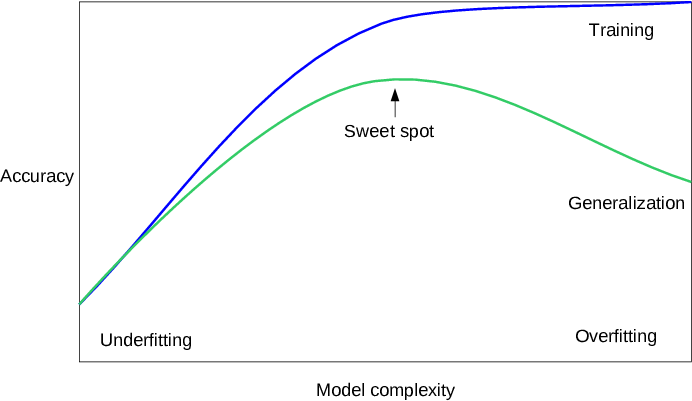
\includegraphics[scale=0.5]{../img/tradeoff_overfitting_underfitting.png}
	\caption{Trade-off tra overfitting e underfitting}
\end{figure}

% TODO: dal libro
\pagebreak

\subsubsection{k-Nearest Neighbour}

Vediamo nello specifico uno dei più semplici algoritmi di machine learning: k-Nearest Neighbor. Questo è un algoritmo utilizzato sia per la classificazione che per la regressione. In entrambi i casi l'algoritmo si basa sul un parametro fissato k il quale indica il numero di vicini da considerare.

Supponiamo di avere due feature (per semplcità), feature 0 e feature 1 le quale descriveranno - insieme all'etichetta - ogni record del nostro dataset. 

Nel caso di classificazione tramite il k-NN, un nuovo elemento non ancora etichettato, (il quale avrà le proprie coordinate (feature0, feature1)), verrà classificato in base al tipo predominante dei suoi vicini. La scelta del k, è quindi l'unica, ma fondamentale scelta per determinare la precisione nella predizione dei futuri elementi da classificare.

In figura 2 viene mostrato come influisce la scelta di differenti parametri k su uno stesso campione C.
\vspace{5 mm}
\begin{figure}[h!]
	\center
	\label{fig:knn_difference}
	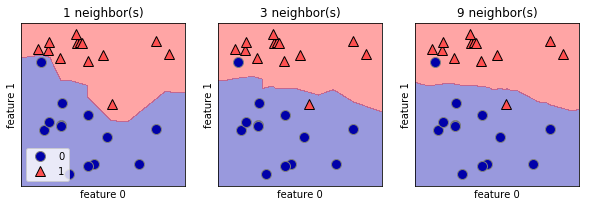
\includegraphics[scale=0.7]{../img/knn_comparison}
	\caption{k-NN classifier con k differenti}
\end{figure}

Questo algoritmo è utilizzato con un k dispari, il quale non permette di avere casi di indecisione e di poter sempre definire a quale classe appartiene.
\pagebreak
\vspace{5 mm}
\begin{figure}[h!]
	\center
	\label{fig:knn_classifier}
	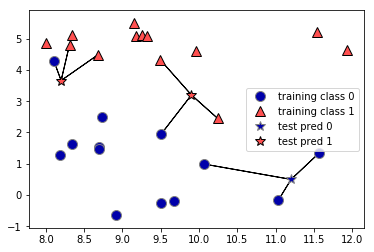
\includegraphics[scale=0.85]{../img/knn_classifier}
	\caption{k-NN classifier}
\end{figure}

Nel caso di regressione tramite il k-NN, il risultato sarà pari alla media del valore target che vogliamo predire di tutti i k vicini. Vediamo un esempio in dettaglio del funzionamento.

\begin{figure}[h!]
	\noindent
	\center
	\label{fig:knn_regressor}
	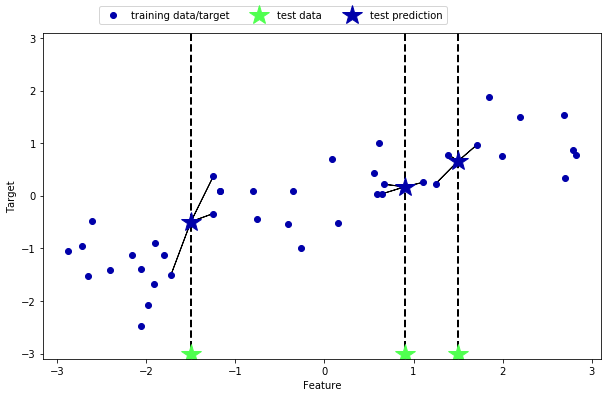
\includegraphics[scale=0.6]{../img/knn_regressor}
	\caption{k-NN regressor}
\end{figure}

\pagebreak

Immaginiamo che nel nostro dataset abbiamo due caratteristiche 'a e 'b per ogni elemento, dove 'a è il valore su cui vogliamo basare il modello e 'b è il valore che siamo interessati a predire. Prendendo ad esempio, un k pari a 3 significherà (come vediamo in figura 1.5) che il nuovo elemento 'elem avrà come valore target la media dei target dei 3 elementi più vicini, sull'asse delle ascisse (ovvero l'asse su cui sono disposti i 'a)
\pagebreak

\subsubsection{Linear models}
I modelli lineari sono una classe di modelli che cercano di effettuare predizioni basandosi su una funzione lineare basata sull'insieme delle feature o caratteristiche appartenenti all'elemento da analizzare. 
Nel caso della regressione, la funzione di cui parliamo è definibile come segue:
\[ y' = w_{0} * x_{0} + w_{1} * x_{1} + ... + w_{n} * x_{n} + b \]


dove $n$ rappresenta il numero di feature, $x$ le feature, $ w $ i pesi da attribuire alle singole feature e la $ b $ rappresenta i parametri attribuiti al modello che si sta allenando.
Prendendo una sola feature (quindi $ n $ pari a 1), $ y' $ risulterebbe:

\[ y' = w_{0} * x_{0} + b\]

la quale è esattamente una funzione di una linea retta, dove w è l'angolo e b è lo scostamento dall'origine degli assi.

Per riprendere l'esempio precedente, supponiamo che si voglia quantificare il numero di giorni necessari per guarire un paziente malato.
Supponiamo, per semplicità, di avere una sola caratteristica definita all'interno della diagnosi che rappresenta l'età del paziente (sull'asse delle ascisse) e per ogni punto il relativo tempo di guarigione - in giorni - (sull'asse delle ordinate). 
Avendo quindi una serie di punti, è possibile tracciare una retta che approssima a tutti i punti definiti nel campione di allenamento (anche chiamato training set). Nell'immagine xxx è illustrata la retta appena citata.

Tutto questo, per quanto riguarda l'utilizzo di modelli lineari nella regressione, nella classificazione invece si mantiene la stessa formula con la piccola differenza che si introducono degli intervalli per definire a quale classe appartiene il singolo caso. Nella classificazione binaria, ad esempio la formula risulterebbe come segue:
\[ y' = w_{0} * x_{0} + w_{1} * x_{1} + ... + w_{n} * x_{n} + b > 0 \]

dove, supponendo di avere le classi "1" e "0", se la $ y' $ fosse maggiore di $ 0 $ appartiene alla classe "1", alla classe "0" altrimenti.

Nella figura xxx è mostrato l'esempio appena citato, dove i cerchi sono la classe 0 e i triangoli la classe 1.

\pagebreak

\subsubsection{Support Vector Classifier}
I SVC (Support Vector Classifier) sono una classe di modelli che si preoccupa di individuare un iperpiano utile a separare (e quindi classificare) i punti nel piano in diversi gruppi, i quali vanno a definire le classi che ci permettono, una volta inseriti i nuovi dati, di attribuire a questi, la rispettiva classe.

Il primo problema che i SVC devono risolvere, è capire quale sia l'iperpiano che suddivide nel modo migliore i dati, questo perchè dati, ad esempio, due gruppi di punti è possibile dividerlo in infiniti modi. 
Una volta presi gli iperpiani candidati, per decidere qual'è il migliore, si prendono i punti P più vicini a questo iperpiano I, i quali vengono definiti vettori di supporto. Per ogni retta R e i relativi vettori di supporto V, viene calcolata la distanza tra R e V la quale indicherà il "margine". Si definisce retta migliore, la retta che riesce a massimizzare il proprio margine dai vettori di supporto. In figura xxx è possibile vedere tutti i componenti dell'SVC in gioco.

[IMMAGINE DI SVC CON TUTTI GLI ATTORI IN GIOCO]

Tutto questo però accade quando abbiamo solamente due dimensioni. Quando ci confrontiamo con dei problemi reali, le feature in gioco che definiscono i punti sono molte, molte di più. Per ovviare a questo problema si ricorre alle funzioni kernel, le quali sono delle funzioni in grado di mappare dei vettori definito in un spazio a n dimensioni, in uno spazio a m dimensioni.
Questo 'trick' del kernel consente di riutilizzare i SVC anche laddove non è possibile suddividere i punti tramite una semplice retta.

Supponiamo di avere un caso mostrato in figura xxx, dove si hanno due sole dimensioni, ma dove non è possibile suddividere i punti con una semplice linea.


Tramite una funzione kernel trasformiamo questi due punti definiti dalle coordinate x e y, in dei punti definiti dalle coordinate x, y e z, in questo modo possiamo rivedere il tutto in 3 dimensioni e tracciare un iperpiano che suddivide correttamente i punti nello spazio a 3 dimensioni, per poi successivamente ridefinirlo secondo le due dimensioni iniziali di partenza.

Come esplicato in un articolo di towards data science (https://towardsdatascience.com/https-medium-com-pupalerushikesh-svm-f4b42800e989), riporto l'esempio esplicativo:

Presi dei punti in uno spazio bidimensionale, ci capita la situazione in cui questi non sono suddivisibili tramite una retta.

[IMMAGINE DEI PUNTI DISPOSTI IN MANIERA NON DIVISIBILE IN UN PIANO A 2 DIMENSIONI]

Aggiungiamo una terza dimensione z e definiamola come segue:
\[ z = x^2 + y^2 \]

Il risultato ottenuto è dato dalla seguente immagine:

[IMMAGINE DEI DATI PLOTTATI SULL'ASSE Z]

Notiamo subito che ora è facile suddividere i punti in due distinti gruppi tramite una retta k (che rispetta il principio delle SVM):

\[ z = k \]

dato che z è stato definito come:

\[ z = x^2 + y^2 \]

poniamo la retta k come segue:

\[ k = x^2 + y^2 \]

il che ci consente di ottenere una linea nello spazio a due dimensioni, che sarà esattamente la nostra divisione tra i gruppi.

Quindi quando ci si trova davanti a problemi n-dimensionali bisogna sempre ricorrere al trucco del kernel. Questo trucco prevede anche dei parametri $ C $ e $ \gamma $, detti parametri di tuning.
Essi influiscono sulla selezione dell'iperpiano che si va ad ottenere nello spazio inziale:
\begin{itemize}
	\item $C$: è il parametro che consente di definire un costo nell'errore della suddivisione dei punti, vale a dire che nel caso in cui si scelga una C grande significa che ogni singolo errore avrà un costo elevato, andando cosi ad adattare il modello SVM il più preciso possibile al training set. Adattando il modello in maniera eccessiva al training set, però, si rischierebbe di andare in overfitting e quindi comporterebbe ad una classificazione errata nel caso di esempi estranei all'insieme dei dati di allenamento. Avendo invece, una C piccola, significa che il costo di errore sarà basso, il quale comporterà che durante l'allenamento del modello, saranno presenti diversi errori di classificazione, però, così facendo si sta generalizzando maggiormente il modello a nuovi casi da etichettare, il che può essere positivo. Come citato sopra, vi rimando al grafico che denota che lo sweetspot, ossia il compromesso per ottenere un buon risultato di predizione, è a metà tra l'underiftting e l'overfitting.
	
	\item $\gamma$
\end{itemize}


\pagebreak

\subsubsection{Alberi di decisione}

Gli alberi di decisione o decision trees, è un algoritmo di classificazione e regressione, che, fondamentalmente, basa la sua logica sull'apprendimento di una struttura, sulla domanda 'se questo allora...'/'altrimenti questo...' fino ad arrivare ad una decisione finale.

Prendo spunto da un esempio fatto nel libro 'Introduction to machine learning' in cui si vuole distinguere un animale tra: falco, pinguino, delfino, orso.
L'algoritmo lavora andando a fare determinate domande a cui puoi rispondere vero o falso, ad esempio, si parte da una domanda che può semplicemente essere: "Ha le piume?". In questo modo si aprono due strade, "ha le piume" e "non ha le piume", suddividendo in due gruppi distinti gli animali. Prendendo gli animali che non hanno le piume (orso e delfino), e facendo un'ulteriore domanda, che differenzia i due animali, si può arrivare a capire di quale animale si sta parlando tramite questa serie di risposte. Seguendo la domanda, "Ha le pinne?", possiamo capire che se la risposta è si, è il delfino, ovvero l'unico animale tra i 4 sopra scelti che non ha le piume e ha le pinne.

Seguendo questa logica è possibile arrivare (con le giuste domande) a dire di quale tipo di animale si sta parlando.

Questo era un semplice esempio che non rispecchia la realtà, e i campi di utilizzo di questo algoritmo. Spesso i dati che vengono analizzati hanno dei valori di tipo continuo, quindi la domanda a cui si risponde, tendenzialmente, è del tipo: "x è maggiore di y?". Questo è il modo in cui operano questi algoritmi in caso di valori di tipo continuo e così facendo si va a costruire un completo albero di decisione.

Come abbiamo già visto anche negli altri algoritmi, il problema dell'overfitting e underfitting è un problema ricorrente e nel caso dell'albero di decisione non è da meno.
Infatti se viene costruito un albero troppo dettagliato e quindi con un livello di profondità eccessivo si va ad adattare in maniera eccessiva (quindi in overfitting) al training set, andando a definire zone anche molto piccole, come viene mostrato in figura xxx.

[IMMAGINE DECISIONN TREE OVERFITTING]

Analizzando un caso simile è possibile vedere in figura xxx come l'errore su un test set (quindi un insieme di dati utile a testare il modello allenato), cresca rispetto al train, questo succede proprio perchè il modello non è generalizzato, ma si è allenato specificandosi in maniera eccessiva al training set.

[IMMAGINE GRAFICO ERRORE SU TEST SET CON OVERFITTING]

Per risolvere questo problema, esistono due strategie:
\begin{itemize}
	\item far terminare lo sviluppo dell'albero dopo pochi passi (pre-potatura): limitare la profondità dell'albero definendo una variabile che tenga conto della prodfondità dell'albero, la quale quando supera una soglia prefissata, interrompe lo sviluppo di questo
	
	\item rimuovendo i nodi che hanno contengono informazioni ridotte (post-potatura)
\end{itemize}

\pagebreak
\subsection{Unsupervised}
Il secondo importante approccio all'applicazione del machine learning, consiste nella tecnica non supervisionata. Cosa si intende dire con non supervisionata? Come può una macchina imparare se nessuno la guida nella scelta di decisioni?
Questa è proprio la sfida che si vuole superare con questa tecnica, ovvero far estrapolare alla macchina, delle informazioni "nascoste" all'interno dei dati che gli vengono forniti. Cercando dei legami o regole che i dati tendono a seguire, all'interno del set datogli in input senza fornire nessun tipo di ifnormazione ulteriore che possa guidare il modello di apprendimento in qualche modo (a differenza, appunto, del modello supervisionato).

Ci sono diversi tipi di machine learning non supervisionato, in questo capitolo ci limiteremo a elencarne la logica che seguono e quale possibile campo di utilizzo, senza entrare troppo nello specifico.

Un primo tipo di Unsupervised learning è il clustering. Il clustering è una tecnica che serve per suddividere in gruppi distinti degli elementi che hanno dati e caratteristiche in comune. Per essere più chiari, vediamo subito un possibile esempio.
Supponiamo di aver scattato una serie di foto i cui soggetti sono delle persone, magari nostri amici o parenti e decidiamo di caricarle su un social network. Durante il caricamento, il social su cui le stiamo caricando, si permette di visionare le foto e applicare proprio un algoritmo di clustering. In che modo? L'algoritmo non sa nè chi siano le persone raffigurate nè quante esse siano. L'algoritmo andrà a cercare tutti i volti nelle foto che abbiamo caricato e successivamente, dopo aver ottenuto una lista di tutti i volti estrapolati da ogni foto, tramite un algoritmo di clustering va a cercare somiglianze in questi volti, andando così a raggruppare le foto dove è presente lo stesso soggetto.

***TODO***: ulteriori esempi
\pagebreak
\subsection{Semi-supervised}

L'approccio semi-supervised, non è un vero e proprio approccio, bensì una tecnica che sta a metà tra le due appena viste (supervisionato e non supervisionato). Questa tecnica consiste nel combinare le due tecniche e quindi fornire un risultato basandosi su un input eterogeneo: etichettato e non.

Questo approccio risulta utile quando si ha una grande mole di dati, e gli utenti che sono in grado di etichettare i dati sono utenti specializzati, quindi, nella situazione reale, non sempre questo è possibile, proprio perchè possono mancare risorse umane competenti o tempistiche adeguate.

Esistono differenti algoritmi per l'apprendimento automatico mediante un sistema semi-supervisionato:
\begin{itemize}
	\item Self training
	\item Multi-view training
	\item Self-ensembling
\end{itemize}

Per quanto riguarda il multi-view training, esso mira a formare diversi modelli con diverse visualizzazioni dei dati. Idealmente, queste viste sono complementari e i modelli possono collaborare per migliorare il risultato finale. Queste viste possono differire in diversi modi, ad esempio nelle funzionalità che utilizzano, nelle architetture dei modelli o nei dati su cui i modelli vengono formati.

Il self-ensembling, come il multi-view training, punta a combinare diverse varianti dei modelli. A differenza però di quest'ultimo, la diversità nei modelli non è un punto chiave perchè il self-ensembling utilizza principalmente un singolo modello in diverse configurazioni al fine di rendere più affidabili le previsioni del modello. 

A titolo di esempio vedremo più in dettaglio l'algoritmo di Self training che è stato uno dei primi ad essere sviluppato ed è l'esempio più diretto di come le previsioni di un modello possono essere incorporate nel training del modello.

L'algoritmo di auto-allenamento prevede quindi di basarsi per quanto può su dei dati che sono stati preventivamente definiti secondo un particolare modo e altri che sono solamente dei dati da studiare e analizzare. Questi ultimi vengono comuqnue utilizzati, ma in maniera più cauta, ovvero, prima di allenare il modello per imparare a fare una predizione sui futuri elementi dati in input, il modello si concentrerà ad etichettare gli input che ancora sono senza alcuna etichetta.

Come viene spiegato in un articolo su ruder.io %[https://ruder.io/semi-supervised/index.html\#relatedmethodsandareas], 
la logica di classificazione dei dati non ancora classificati segue quanto scritto:		\\
"Formalmente, l'auto etichettamento avviene su un modello M avente un training set etichetto L con delle etichette contenute in C e un set non etichettato U. Ad ogni iterazione, per ogni x in U, il modello fornisce delle predizioni su m(x) sottoforma di probabilità p(x, c) ovvero probabilità che x appartenga alla classe c per ogni c in C. Tra le probabilità appena calcolate, definiamo P(x, c) come la probabilità avente il valore maggiore, allora se P è maggiore di una soglia T, x verrà aggiunto a L con l'etichetta c. Questo processo viene ripetuto per un numero fisso di iterazioni o fino a quando non ci sono più dati da etichettare.".[nota: traduzione libera del testo: nell'originale è presente una formula ceh io rendo a parole]

Di seguito vediamo uno pseduo-codice che segue quanto detto sopra:

\begin{algorithmic}[1]
	\Repeat
	\State $m \gets train\_model(L)$
	\For {$x \in U$}
	\If {$\max m(x) > \tau$}
	\State $L \gets L \cup \{(x, p(x))\}$
	\EndIf
	\EndFor
	\Until {no more predictions are confident}
\end{algorithmic}

\pagebreak
\subsection{Reinforcement learning}
Il quarto ed ultimo approccio chiamato Reinforcement learning, è un approccio che si differenzia da quelli visti fino ad ora. Questo paradigma si occupa di problemi di decisioni sequenziali, in cui l'azione da compiere dipende dallo stato attuale del sistema e ne determina quello futuro. In altre parole, questo è un sistema dinamico che può apprendere in seguito ad ogni decisione presa, a prescindere che questa sia giusta o sbagliata.

\begin{figure}[h!]
	\noindent
	\center
	\label{fig:rl_scenario}
	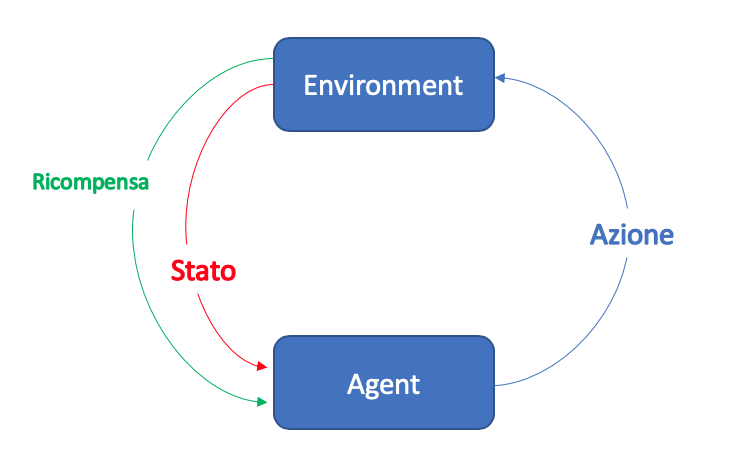
\includegraphics[scale=0.5]{../img/rl_scenario}
	\caption{Scenario RL}
\end{figure}
 (https://www.aitrends.com/education/udacitys-school-of-ai-opens-the-new-deep-reinforcement-learning-nanodegree-program-for-enrollment/) (https://www.guru99.com/reinforcement-learning-tutorial.html)

Quando il sistema prende una decisione, esso otterrà una "ricompensa" che può essere un punteggio, che sarà alto o basso a seconda se la decisione presa è giusta o sbagliata. Con questa logica, la macchina cercherà di fare sempre meglio per arrivare a ottenere il punteggio più alto possibile, prendendo così solo le decisioni corrette. 

Di seguito, sono citati dei casi di utilizzo di questo approccio:

\begin{itemize}
	\item Imparare a giocare a scacchi
	\item Imparare a guidare un veicolo
\end{itemize}

% 
%			CAPITOLO 2: Stato dell'arte
% 

\chapter{Stato dell'arte}
\label{chap:stato_arte}


Una delle domande più ricorrenti da parte degli studenti \`e cosa si intenda per ``stato dell'arte''. Concretamente, si tratta di individuare la situazione corrente riguardo la tematica trattata nell'elaborato. A titolo di esempio, se il lavoro di tesi si concentra su un (presunto) innovativo algoritmo per suggerire i brani di una playlist, è necessario verificare che tale approccio sia veramente innovativo e, in ogni caso, studiare gli approcci alternativi già disponibili in letteratura.

Per ottenere tale risultato, è necessario condurre ricerche approfondite a livello bibliografico (testi di riferimento, articoli scientifici, ecc.) e implementativo (sul web, sugli store, ecc.) \textbf{prima} di iniziare il proprio lavoro.

\section{Risorse}

Riguardo gli articoli scientifici, si caldeggia l'uso del motore di ricerca specializzato Google Scholar.\footnote{\url{https://scholar.google.it/}.} Esistono, poi, numerosi repository che consentono di accedere gratuitamente a pubblicazioni scientifiche, tra cui ResearchGate,\footnote{\url{https://www.researchgate.net/}} Zenodo,\footnote{\url{https://zenodo.org/}} e SBA - Sistema Bibliotecario di Ateneo,\footnote{\url{http://www.sba.unimi.it/index.html} con contenuti scaricabili solo dalla rete interna all'ateneo.}

\`E importante riconoscere, nella grande mole di letteratura scientifica disponibile, i lavori pi\`u autorevoli e affidabili. Un primo elemento per orientarsi \`e che non tutte le sedi di pubblicazione sono uguali. In particolora una regola generale (per quanto non assoluta) \`e che gli articoli pubblicati su {\em rivista} sono tipicamente pi\`u completi e rigorosi di quelli pubblicati su atti di {\em convegno}. Un secondo elemento correlato all'autorevolezza della pubblicazione \`e il numero di citazioni che questa ha raccolto da parte di altri ricercatori (dato visibile ad esempio su Google Scholar). Infine, \`e opportuno riconoscere le sedi di pubblicazione (riviste e convegni) rilevanti per il settore: per l'informatica musicale, un primo riferimento pu\`o essere la lista di riviste e di convegni disponibile sul sito dell'associazione Sound and Music Computing.\footnote{\url{http://www.smcnetwork.org}}

\section{Buone pratiche}

Alcuni consigli di buone pratiche per l'analisi dello stato dell'arte.
\begin{itemize}
\item Imparare a leggere in maniera {\em efficace}. Ci sono migliaia di articoli potenzialmente interessanti, quindi \`e essenziale riuscire a estrarre in breve tempo gli elementi rilevanti di un articolo senza perdersi nei dettagli (fino a che non sia strettamente necessario), nonch\'e annotare in maniera ordinata tali elementi.
\item Imparare a leggere in maniera {\em critica}. Raramente un articolo scientifico \`e perfetto, gli aspetti tecnici e gli eventuali punti deboli (metodologie, ripetibilit\`a dei risultati, ecc.) vanno valutati e annotati con attenzione.
\item Imparare a seguire le ``piste'' interessanti. Una volta trovato un articolo rilevante, \`e utile esaminare
\begin{itemize}
\item gli articoli che esso cita (i suoi riferimenti bibliografici): questo permette di rintracciare riferimenti autorevoli a cui l'articolo si appoggia;
\item gli articoli che lo citano (ad esempio Google Scholar offre questa funzionalit\`a): questo permette di rintracciare riferimenti pi\`u recenti che hanno proseguito nella stessa direzione di ricerca.
\end{itemize}
\item Imparare a lavorare iterativamente.
\begin{itemize}
\item Aggiungere alla propria bibliografia gli articoli considerati rilevanti, a mano a mano che vengono trovati.
\item Raggrupparli iterativamente in sottotematiche.
\item Usare inizialmente un approccio ``inclusivo'' (nel dubbio, aggiungere un articolo in bibliografia piuttosto che scartarlo), e solo in un secondo tempo decidere cosa tenere e cosa scartare.
\end{itemize}
\end{itemize}



\section{Bibliografia e sitografia}
\label{sec:biblio}

La bibliografia di un lavoro scientifico deve necessariamente essere ricca. Tutti i testi in bibliografia devono essere citati almeno una volta nel corso dell'elaborato. 

Nella valutazione della bibliografia da parte della commissione, i testi cartacei sono considerati significativamente più validi dei siti consultati. Ne consegue che la bibliografia debba essere ricca di testi pubblicati, siano essi libri, articoli, al limite tesi di laurea o di dottorato o rapporti tecnici. Si suggerisce di evitare citazioni a fonti di dubbia valenza scientifica, quali Wikipedia, W3Schools, ecc.

Se è necessario citare siti Web, esistono tre strade ugualmente accettabili:
\begin{enumerate}
	\item se il numero di siti non è preponderante rispetto ai testi ``tradizionali'', è possibile inserirli parimenti in bibliografia;
	\item se i siti da citare sono numerosi, è più opportuno creare una sorta di bibliografia parallela e separata, detta \textit{sitografia};
	\item infine, se la citazione dei siti serve a individuare un prodotto e non una fonte di informazioni, la soluzione più opportuna è quella delle note a piè di pagina.
\end{enumerate}





% 
%			CAPITOLO 3: Tecnologie utilizzate
% 

\chapter{Tecnologie utilizzate}
\label{cap3}

In questo capitolo vengono presentati alcuni suggerimenti utili per un utente \LaTeX\ alle prime armi.


\section{Generalit\`a}

\subsection{La scrittura WYSIWYG vs.\ WYSIWYM}

L'acronimo WYSIWYG sta per ``What You See is What You Get'', e si riferisce al concetto di ottenere sulla carta testo e immagini che abbiano una disposizione grafica equivalente a quella visualizzata a schermo dal software di videoscrittura. Un esempio classico di WYSIWYG è Microsoft Word, che mostra il testo impaginato e formattato come ci si aspetta di vederlo una volta stampato.

L'acronimo WYSIWYM sta per ``What You See is What You Mean'', ed è il paradigma per la creazione di testi strutturati. \LaTeX\ è un ambiente che supporta tale paradigma. In realtà, anche Microsoft Word avrebbe la possibilità di strutturare il testo, principalmente attraverso il meccanismo degli stili, ma pochissimi utenti sfruttano tale funzionalità (ovviamente se sceglierete di scrivere la tesi in Word raccomandiamo caldamente l'uso di tali funzioni).

I principali svantaggi di un sistema WYSIWYM sono il tempo di apprendimento, dovuto a una minore intuitività degli strumenti software, e la necessità di invocare la compilazione del documento per vederne l'aspetto definitivo. Ad esempio, in \LaTeX\ l'intero documento viene scritto in testo semplice, che all'interno contiene ambienti e comandi con informazioni di layout, e solo la compilazione permette di scoprire eventuali errori di sintassi e giungere, infine, alla creazione del PDF. 

Le difficoltà iniziali, però, sono ampiamente compensate dai vantaggi a medio e lungo termine. Infatti, il lavoro risulterà perfettamente impaginato e strutturato, e dunque avrà un aspetto professionale. Questo riguarda non solo gli stili, che vengono applicati al testo in modo coerente con il template prescelto, ma anche problemi tipicamente spinosi di Word, quali il posizionamento delle immagini e delle tabelle, la creazione di una bibliografia con relative citazioni nel testo, la creazione di un sommario (per cui esistono funzioni automatiche, ma sono piuttosto macchinose). Diventa automatico e molto semplice, ad esempio, aggiungere un indice delle figure o delle tabelle, oppure numerare le formule espresse nel testo. Un altro aspetto su cui \LaTeX\ è nettamente superiore a Word è proprio la scrittura di formule matematiche, come mostrato nell'esempio qui riportato:
\begin{equation}
x_i(n) = a_{i1}u_1(n) + a_{i2}u_2(n) + \cdots + a_{iJ}u_J(n) \, .
\label{eq:multimix}
\end{equation}

\subsection{Risorse e strumenti}

Esiste una vastissima gamma di risorse online per avvicinarsi a \LaTeX. Un buon punto di partenza \`e la lista messa a disposizione sul sito del \TeX\ Users Group (TUG).\footnote{\url{http://www.tug.org/interest.html}}
Tra queste si consiglia in particolare la ``Not so Short Introduction to LaTeX2e'',\footnote{\url{http://mirrors.ibiblio.org/CTAN/info/lshort/}}. Per chi volesse approfondire, uno dei riferimenti bibliografici pi\`u completi \`e il libro di Mittelbach {\em et al.}~\cite{mittelbach2004latex}.

In alternativa a un'installazione locale sul proprio pc, \`e possibile utilizzare un editor \LaTeX\ online, con il vantaggio di avere immediatamente a disposizione l'ambiente di sviluppo e tutti i package necessari, nonch\'e di potere condividere il proprio progetto con il relatore di tesi. Il pi\`u diffuso editor \LaTeX\ online \`e Overleaf,\footnote{\url{http://www.overleaf.com}} dove si pu\`o trovare anche ulteriore documentazione (in particolare la guida ``Learn \LaTeX\ in 30 minutes'').\footnote{\url{https://www.overleaf.com/learn}}

Qualunque sia la risorsa utilizzata, ecco un elenco non esaustivo di argomenti di base nei quali con tutta probabilit\`a ci si imbatter\`a durante la stesura della tesi.
\begin{itemize}
\item Formattazione del testo (grassetto, italics, dimensioni font, ecc.) e del documento (paragrafi, comandi \verb|\chapter|, \verb|\section|, \verb|\tableofcontents|, ecc.).
\item Elenchi: ambienti {\em itemize} e {\em enumerate}, pacchetti rilevanti ({\em paralist})
\item Riferimenti incrociati: comandi \verb|\ref|, \verb|\pageref| e \verb|\label|, etichette.
\item Matematica: equazioni, modalit\`a {\em inline} e {\em displayed}, pacchetti rilevanti ({\em amssymb}, {\em amsmath}).
\item Figure: formati grafici, ambiente {\em figure}, pacchetti rilevanti ({\em graphicx}, {\em subfloats} per figure multiple).
\item Tabelle: ambienti {\em table} e {\em tabular}, pacchetti rilevanti ({\em array}, {\em multirow}, {\em longtable}).
\item Riferimenti e bibliografie (si veda pi\`u sotto la sezione~\ref{sec:bibtex}).
\end{itemize}

\section{Suggerimenti sull'uso di \LaTeX}
\label{sec:consigli_latex}

Fatte salve le indicazioni generali fornite nella sezione precedente, di seguito si riportano alcune osservazioni puntuali sulle domande e gli errori pi\`u tipici degli studenti alle prime armi con \LaTeX.

\subsection{Riferimenti incrociati}

Uno dei principali vantaggi di \LaTeX\ è la possibilità di impostare riferimenti automatici a molti elementi del documento, tra cui capitoli, sezioni, sottosezioni, tabelle, figure, equazioni, riferimenti bibliografici, e via dicendo.

Quindi il modo corretto per riferirsi, ad esempio, al secondo capitolo non è scrivere ``Capitolo 2'' bensì ``Capitolo~\ref{chap:stato_arte}''. Il risultato apparente (nel PDF) è lo stesso, mentre ci sono differenze sostanziali a livello di codice. Il vantaggio è che, se il secondo capitolo diventasse il terzo, il riferimento incrociato continuerebbe a puntare alla posizione corretta. Si pensi, per estensione, alla numerazione delle immagini, o ai riferimenti alla bibliografia.

Sintatticamente, questo richiede di inserire dei comandi \verb|\label{mia_label}| all'interno degli elementi cui ci si vuole riferire, e dei comandi \verb|\ref{mia_label}| dove si vuole creare il riferimento. Fa eccezione la bibliografia (si veda pi\`u sotto la sezione~\ref{sec:bibtex}).


\subsection{Ritorni a capo}

I ritorni a capo in \LaTeX\ possono essere effettuati in due modi: con la sintassi \verb|\\| o con una doppia pressione del tasto di ritorno a capo. In generale, la soluzione corretta è la seconda, che equivale a usare il tasto Enter in Word. Il doppio Backslash, che corrisponde a Shift+Enter in Word, crea una nuova riga senza interruzione del paragrafo. Questo va usato solo in casi molto specifici, come nella frase seguente.

Il sito web ufficiale del Laboratorio di Informatica Musicale è:\\
\url{https://www.lim.di.unimi.it}.

In molti stili di \LaTeX, un nuovo paragrafo (dopo un doppio a capo) crea un rientro della prima riga. Non c'\`e nulla di male nel rientro, ma se proprio lo si vuole evitare la soluzione \textbf{non} \`e usare il doppio BackSlash! Esistono molte soluzioni pi\`u appropriate (ad esempio, dare una dimensione nulla al rientro tramite il comando \verb|\setlength{\parindent}{0ex}|, da inserire nel preambolo della tesi).

\subsection{Accenti}

Scrivendo la tesi in italiano, l'uso di lettere accentate \`e frequente. I caratteri accentati immessi da tastiera non vengono per\`o riconosciuti nativamente. Invece l'accento grave e acuto in \LaTeX\ si ottengono rispettivamente con i comandi \verb|\`{a}| e \verb|\'{a}.| 

In alternativa \`e possibile specificare che si usa la codifica UTF-8, usando il comando \verb|\usepackage[utf8]{inputenc}| nel preambolo del documento (già incluso in questo template). In questo modo i caratteri accentati immessi da tastiera verranno riconosciuti.

Nota ortografica: attenzione a non sbagliare gli accenti: si scrive ``\`e'', ma si scrive ``perch\'e''.

\subsection{Spazi tra parole}

Riguardo la gestione della spaziatura tra parole, \LaTeX\ adotta una strategia molto elegante, che lascia uno spazio maggiorato dopo il punto di fine periodo. Un potenziale problema è che questo spazio extra viene introdotto dopo qualsiasi occorrenza del punto, indipendentemente dalla funzione sintattica, e dunque anche dopo i nomi puntati, quali ``R. Schumann'', o dopo le formule ``ad es.'', ``Fig. n'', ``ecc.'' e via dicendo. Per evitarlo, questi spazi da non aumentare vanno sostituiti con alternative, quali un Backslash seguito da uno spazio (che immette un \textit{control space}) o una tilde \verb|~| (che introduce un \textit{unbreakable space}, utile a impedire ritorni a capo intermedi).\footnote{Per una trattazione completa delle numerose varianti, si veda \url{https://tex.stackexchange.com/questions/74353/what-commands-are-there-for-horizontal-spacing}}

\subsection{Interlinea}

Per aumentare la leggibilit\`a della tesi pu\`o essere utile usare un'interlinea maggiore di 1. Un modo per ottenerlo \`e usare il comando \verb|\linespread{1.6}| nel preambolo del documento. Nota: il valore $1.6$ indica interlinea doppia, il valore $1.3$ indica interlinea 1.5. Don'ask why.


\subsection{Doppie virgolette}

L'uso dell'unico carattere di doppie virgolette presente sulla tastiera è assolutamente sconsigliato, in quanto non viene correttamente interpretato da \LaTeX, soprattutto riguardo l'apertura delle virgolette.

La combinazione giusta da utilizzare è \verb|``| per l'apertura e \verb|''| per la chiusura. Si noti che in entrambi i casi si tratta di doppi apostrofi ravvicinati, e non di singoli caratteri. Se si utilizza come editor TeXstudio, c'è un'opzione per sostituire automaticamente le doppie virgolette con la versione corretta in \LaTeX: Opzioni $\rightarrow$ Configura TeXstudio... $\rightarrow$ Editore $\rightarrow$ Sostituisci i doppi apici: Inglesi.

Le virgolette caporali, o francesi, si ottengono con i comandi \verb|\guillemotleft| e \verb|\guillemotright|, il cui risultato è \guillemotleft questo\guillemotright.


\subsection{Ambienti per scrivere codice}

Il codice all'interno dell'elaborato va scritto con carattere monospaziato e rispettando, nell'ambito del possibile, le originali regole (o buone pratiche) di indentazione.

Per farlo, esiste innanzi tutto l'ambiente verbatim, che va aperto e chiuso con i comandi \verb|\begin{verbatim}| ed \verb|\end{verbatim}|.

Tra le alternative, si segnala l'ambiente lstlisting, che richiede innanzi tutto di aggiungere nel preambolo \verb|\usepackage{listings}|, e quindi di aprire e chiudere l'ambiente con i comandi \verb|\begin{lstlisting}| ed \verb|\end{lstlisting}|. Un esempio, relativo al calcolo del massimo comun divisore attraverso l'algoritmo di Euclide in Python, è:

\begin{lstlisting}
def MCD(a,b):
	while b != 0:
		a, b = b, a % b
	return a
\end{lstlisting}

Se dopo l'apertura dell'ambiente si specifica tra parentesi quadrate il linguaggio adottato, ad esempio con la sintassi \verb|\begin{lstlisting}[language=Python]|, si ottiene automaticamente l'evidenziazione del codice:

\begin{lstlisting}[language=Python]
def MCD(a,b):
	while b != 0:
		a, b = b, a % b
	return a
\end{lstlisting}

L'elenco dei linguaggi supportati e le opzioni avanzate per personalizzare la visualizzazione del codice si trovano all'indirizzo \url{https://www.overleaf.com/learn/latex/Code_listing#Reference_guide}.

Infine, si consideri la possibilità di importare interi file di codice attraverso la sintassi \verb|\lstinputlisting[language=nomelinguaggio]{filesorgente}|.

\subsection{Figure}

In tutti i casi in cui sia possibile (schemi a blocchi, plot di dati, ecc.), \`e opportuno che le figure siano in formato vettoriale (eps, pdf) per aumentarne la leggibilit\`a.
Nel caso di figure prodotte da software esterno (ad esempio, grafici esportati in eps o pdf da Matlab), \`e consigliabile conservare tutti i sorgenti e i dati utilizzati per generarle: in questo modo sarà possibile ricreare le figure quando necessario.




\section{\hologo{BibTeX}}
\label{sec:bibtex}

\subsection{Generalit\`a}

Esistono più modi per inserire una bibliografia in \LaTeX. Si consiglia fortemente l'utilizzo del sistema \hologo{BibTeX}. Questo consente di aggiungere, rimuovere e modificare voci di bibliografia in maniera efficiente, di formattarle, di riordinarle a piacere e aggiornare automaticamente i corrispondenti riferimenti nel testo, ecc.

Una guida introduttiva e completa \`e ``Tame the BeaST''.\footnote{Accessibile da \url{http://www.tug.org/interest.html}} 
In estrema sintesi, i passi per gestire una bibliografia tramite \hologo{BibTeX} sono essenzialmente tre.
\begin{enumerate}
\item Salvare i riferimenti bibliografici come entry di uno o pi\`u file con l'estensione .bib (si veda ad esempio il file \texttt{bibliografia.bib}, parte di questo template). Gli entry sono scritti in un formato specifico, in particolare ogni entry ha una propria etichetta testuale che lo identifica univocamente.
\item Creare la bibliografia alla fine del documento o dove desiderato, usando il comando \verb|\bibliography{file1.bib,file2.bib,...}|. \`E possibile inoltre specificare uno stile bibliografico attraverso il comando \verb|\biblographystyle{...}|.
\item All'interno del testo, riferirsi a una voce di bibliografia tramite il comando \verb|\cite{etichetta_entry}|. Si noti che una voce bibliografica non viene inclusa in bibliografia in assenza di una citazione all'interno del testo (coerentemente con quanto discusso nella sezione~\ref{sec:biblio}).
\end{enumerate}

\`E consigliabile cominciare a costruire la propria bibliografia in formato bib a mano a mano che si analizza lo stato dell'arte, invece che rimandare alla stesura finale della tesi.

\subsection{Strumenti}

Un file .bib \`e un file di testo e pu\`o quindi essere gestito con un qualsiasi text editor. Esistono comunque molti tool pi\`u evoluti per gestire bibliografie in formato bib. Un'applicazione installabile localmente sul proprio pc \`e JabRef.\footnote{\url{http://www.jabref.org/}}. Oppure esistono tool online, come Zotero,\footnote{\url{http://www.zotero.org/}} che forniscono molte funzionalità tra cui l'esportazione di bibliografie in formato bib.

Peraltro, anche Google Scholar esporta automaticamente citazioni in formato bib cliccando sul link Cita (icona con doppie virgolette) e scegliendo l'opzione \hologo{BibTeX} nella parte bassa della finestra che si apre. \textbf{Attenzione} per\`o: spesso i bib esportati da Scholar sono incompleti o sporchi, \`e sempre consigliabile controllarne la correttezza.

I pi\`u ``smanettoni'' possono addentrarsi a piacere in funzionalit\`a avanzate. Ad esempio \`e possibile creare bibliografie multiple.\footnote{Un possibile modo viene illustrato qui: \url{https://bit.ly/2wI3Y7p}}
Esiste anche il pacchetto \texttt{biblatex}, che fornisce una reimplementazione completa delle funzionalit\`a bibliografiche di \LaTeX-\hologo{BibTeX}, offrendo maggiore flessibilit\`a e mantenendo compatibilit\`a all'indietro con il formato bib.





% 
%			CAPITOLO 4: Il lavoro svolto
% 

\chapter{Nome del Progetto}
\label{cap4}

In genere il capitolo più corposo dell'elaborato è quello in cui si parla del lavoro svolto. Esistono alcune buone pratiche per rendere l'esposizione efficace, eccone alcune.

\section{Panoramica del progetto}

Prima di addentrarsi nei dettagli è bene fornire una panoramica (anche molto schematica, corredata da un diagramma) del lavoro svolto, in modo che il lettore abbia una mappa concettuale con cui orientarsi.

\section{Implementazione}

Una volta fornita una panoramica, è possibile addentrarsi nei dettagli, ricordando che si sta scrivendo un articolo scientifico e non un testo di narrativa. Vanno dunque evitate domande retoriche quali ``\textit{ma come è stato possibile risolvere questo problema? Ebbene \ldots}''.

Vale la pena riportare nel testo solo le parti di codice più importanti, demandando all'appendice il codice completo e altri extra come il manuale utente.

% 
%			CAPITOLO 5: Test
% 

\chapter{Test}
\label{cap5}

Ogni lavoro scientifico richiede una validazione dei risultati ottenuti. Questo si può fare confrontando in modo sistematico il proprio lavoro con lavori concorrenti o misurando l'efficacia del lavoro mediante test con gli utenti. \`E fondamentale che questi test siano ripetibili, dovrete dunque fornire tutti i dettagli necessari nel testo per permettere a chi legge la tesi di replicare l'esperimento.

Progettare e condurre un test soggettivo con utenti \`e un lavoro complesso e lungo, che richiede pianificazione e competenza. Il bel libro di Lazar {\em et al.}~\cite{lazar2017methods} illustra in dettaglio i concetti principali della ricerca sperimentale e le metodologie correlate: ipotesi di ricerca, design sperimentale, analisi dei risultati sperimentali. Quelli che seguono sono alcuni consigli specifici sugli aspetti pi\`u importanti.

\section{Protocollo}

Uno degli errori più comuni è sottovalutare lo studio di un \textit{protocollo} sperimentale. Affinché i risultati dei test siano significativi è necessario non trascurare i seguenti aspetti:

\begin{itemize}
	\item eliminare distorsioni sistematiche involontarie;
	\item isolare le variabili oggetto dello studio;
	\item garantire una numerosità sufficiente del campione;
	\item confrontare gli effetti con un gruppo di controllo.
\end{itemize}

\section{Risultati}

I risultati dei test vanno presentati in modo chiaro e completo, possibilmente indicando la significatività statistica di quanto ottenuto.

\`E buona norma fornire sia i dati numerici (un esempio di come si fanno le tabelle in \LaTeX\  è visibile in Tab.\ \ref{tab:sample}), sia una rappresentazione grafica (a barre, a scatole e baffi, a violino, di dispersione, ecc.).

\`E inoltre consigliato riportare in appendice i dati grezzi completi, in modo da permettere al lettore di ripetere eventuali test statistici.

\begin{table}
	\centering
    \begin{tabular}{|l|l|l|}
	\hline
	Colonna 1 & Colonna 2 & Colonna 3 \\ \hline
	5         & 8         & 1         \\
	6         & 9         & 2         \\
	7         & 0         & 3         \\ \hline
\end{tabular}
	\caption{Tabella di esempio.}
	\label{tab:sample}
\end{table}

\section{Osservazioni}

Quando si traggono conclusioni dai dati bisogna prestare attenzione a non confondere la correlazione con un rapporto di causalità. Molto spesso accade che un test suggerisca la presenza di un fenomeno, ma non dica nulla sulla causa. In questo caso bisogna formulare delle ipotesi, calcolare le implicazioni, ed eseguire un test che valuti se e quali di queste implicazioni si verifichino. Se il nuovo test falsifica la teoria, non importa quanto questa sia elegante: è falsa. Se invece il nuovo test non falsifica la teoria, allora la si può dare per ``vera fino a prova contraria''.

Per queste ragioni è necessario esporre le proprie osservazioni in maniera cauta, senza andare oltre ciò che suggeriscono i dati. \`E certamente possibile speculare sulle cause, ma va esplicitato chiaramente, e tali speculazioni vanno supportate dalla bibliografia.

% 
%			CAPITOLO 6: Conclusioni e sviluppi futuri
% 

\chapter{Conclusioni}
\label{cap6}

\section{Conclusioni}

Nelle conclusioni si tirano le somme di quanto realizzato, facendo un riassunto stringato del lavoro svolto. In particolare vanno dichiarati punti di forza e criticità della ricerca effettuata, nonché quali aspetti dello stato dell'arte siano stati superati dal lavoro in oggetto.

\section{Sviluppi futuri}

Tra gli sviluppi futuri in genere trovano posto quelle migliorie non realizzate per mancanza di tempo, la cui necessità è emersa solo dopo i test, e che riguardano il progetto ad un livello di astrazione più alto (nel caso di tesi che si inquadrano in una linea di ricerca).


% 
%			APENDICE: materiali aggiuntivi e dimostrazioni
% 

\appendix

\chapter{Il tirocinio e la correzione}

Lo studente che si appresta a svolgere il lavoro di tesi generalmente incontra relatore e correlatore a inizio progetto per definire una tabella di marcia, quindi al completamento di ogni obiettivo fissato si ripresenta per un aggiornamento e un controllo. Questo è molto importante per approcciare il problema in modo organico e per evitare di illudersi di aver raggiunto un risultato sufficiente ritenendo concluso il lavoro.

Durante il lavoro è consigliato di prendere appunti su ciò che si sta facendo, in modo da avere una base per la stesura dell'elaborato.

Infine, è richiesto agli studenti di consegnare la proposta di indice prima di iniziare la stesura, per poi consegnare ogni capitolo a mano a mano che questi vengono completati. La tesi completa va consegnata per la rilettura finale a relatore e correlatore almeno una settimana prima della consegna ufficiale, per permettere un ultimo \textit{proof reading} e l'integrazione delle eventuali modifiche richieste.

\chapter{Il riassunto}

In prossimità della data di laurea, viene richiesto agli studenti di caricare in piattaforma anche il riassunto. La sua funzione è permettere alla commissione di visionare rapidamente gli argomenti trattati da ciascun elaborato.

L'estensione di tale documento non dovrebbe superare le due pagine, e spesso una pagina è più che adeguata allo scopo. Riguardo i contenuti, il riassunto riprende -- in maniera molto succinta -- lo schema dell'elaborato finale, e quindi, ad esempio, la scaletta proposta in \ref{sec:organizzazione}.

Visto lo scopo del documento, è buona prassi bilanciare il testo in modo da dedicare poche righe allo stato dell'arte, in favore delle parti originali dell'elaborato.


\chapter{La consegna}

I membri del LIM in generale non richiedono agli studenti di consegnare una copia cartacea del proprio lavoro. In prossimità della discussione viene richiesto loro di condividere in formato digitale:

\begin{itemize}
	\item la versione finale dell'elaborato;
	\item il riassunto caricato in piattaforma;
	\item il codice sviluppato;
	\item tutti i materiali di supporto utilizzati e/o prodotti;
	\item la presentazione predisposta per la discussione.
\end{itemize}

La consegna può avvenire su supporto ottico, via chiavetta USB o attraverso i sistemi di condivisione dei file (WeTransfer, Dropbox, Google Drive, ecc.).



\chapter{La presentazione}

Gli studenti delle lauree triennali hanno a disposizione al massimo 10 minuti per presentare il proprio elaborato, che diventano 15 per le lauree magistrali. 

Si raccomanda di provare ripetutamente il discorso cronometrandosi e considerando i tempi morti per l'accensione del PC, l'avvio dei software, il passaggio da un'applicazione a un'altra, e via dicendo. Si segnala inoltre la possibilità di prenotare l'aula della discussione per provare in anticipo i collegamenti e verificare che immagini e audio vengano correttamente riprodotti.

Per via degli stringenti vincoli temporali, difficilmente una presentazione multimediale può superare la soglia di 15 slide. Questo valore è puramente indicativo, perché dipende dalla densità di informazioni della slide e dal tempo dedicato a ciascuna slide mentre si sta presentando.

La scelta tecnologica più comune è Microsoft PowerPoint, ma qualsiasi alternativa (Prezi, Acrobat PDF, \LaTeX, ecc.) è ammissibile. 

Gli errori più comuni da evitare sono:

\begin{itemize}
	\item slide dal contenuto testuale troppo ricco;
	\item slide che verranno lette parola per parola in fase di presentazione.
\end{itemize}

Entrambi i problemi si risolvono impostando il testo in maniera estremamente schematica, tendenzialmente per elenchi puntati. Si presti attenzione, però, a usare una forma omogenea. 
Ad esempio, sarebbe poco elegante il seguente elenco, che include aggettivi, sostantivi e frasi di senso compiuto, e non fa un uso corretto di iniziali maiuscole:

\begin{itemize}
	\item applicativo esteticamente molto gradevole;
	\item C'è la possibilità di interagire con altri utenti;
	\item l'utente può esportare file in formato XML.
\end{itemize}

Una possibile revisione, basata solo sui sostantivi, è: 

\begin{itemize}
	\item qualità estetica;
	\item interazione tra utenti;
	\item supporto dell'XML.
\end{itemize}

Un altro consiglio per rendere la presentazione cognitivamente più gestibile da parte del pubblico è quello di aggiungere in calce ad ogni slide un indicatore dello stato di avanzamento (ad esempio ``Slide 3 di 15''). In questo modo, in caso di esaurimento del tempo concesso la commissione saprà se dare modo di concludere (``Slide 14 di 15'') o se fermare il candidato (``Slide 14 di 138''). In assenza di un indicatore la commissione tende a presupporre il secondo caso.

Per quanto riguarda gli argomenti da trattare durante la discussione, è opportuno esporre brevemente lo stato dell'arte per concentrarsi sul proprio lavoro, sui test e sui risultati. Una tecnica per capire quanto tempo dedicare a ogni argomento consiste nel dare un peso a ciascuna parte di cui si vuole parlare, quindi assegnare un numero di minuti proporzionale a detto peso in modo da raggiungere il tempo massimo a disposizione.

Video dimostrativi e \textit{live demo} sono gradite, ma è sconsigliabile dedicare troppo tempo a questi contributi, a meno che al contenuto multimediale si sovrapponga una spiegazione da parte del candidato.

%
%			BIBLIOGRAFIA
%

\bibliographystyle{unsrt}
\bibliography{bibliografia}
\addcontentsline{toc}{chapter}{Bibliografia}


% Pagina dichiusura del LIM
\closingpage

\end{document}


 
